\section{Application Structure}

The structure of \projectname{} is a bit different from other web applications.

\subsection{Architecture}

The architecture of \projectname{} differs from other web applications in the way that there exists two different type of servers. The server where the web application is running is called Master after this denoted M.
For each drone in the system there is a Slave denoted S. 
On both M and S there exists daemons which is responsible for different tasks, however there is some similarity that is that these tasks can happen at anytime therefore the program needs to be running at anytime. These daemons are denoted D.
Each user have a browser they view the application through this is denoted B.
It is M's responsibility to communicate with every S in the system.
S is responsible for all communication with the drone it is parred with.
When a new drone is added to the system a new S is setup at the drones location. When this S is up and running it will start to communicate back to M. In this way M will be informed that a new drone have entered the system. M will add the IP of S and the unique name of S's drone to its database.
If the drone already exists in M's database all old session keys will be destroyed, if any exists, and M updates the IP of S if it differs from the old IP. The sessions is destroyed because if there exists one or more sessions to S and it start to communicate that it is online then it is safe to assume that S disconnected or crashed and all old session keys is invalid.

If a user decides that they want to stream from a drone or control it the setup will behave differently. A session key will be made for the user and with this key it is possible to communicate directly with S.

\begin{figure}[htb]
    \centering 
    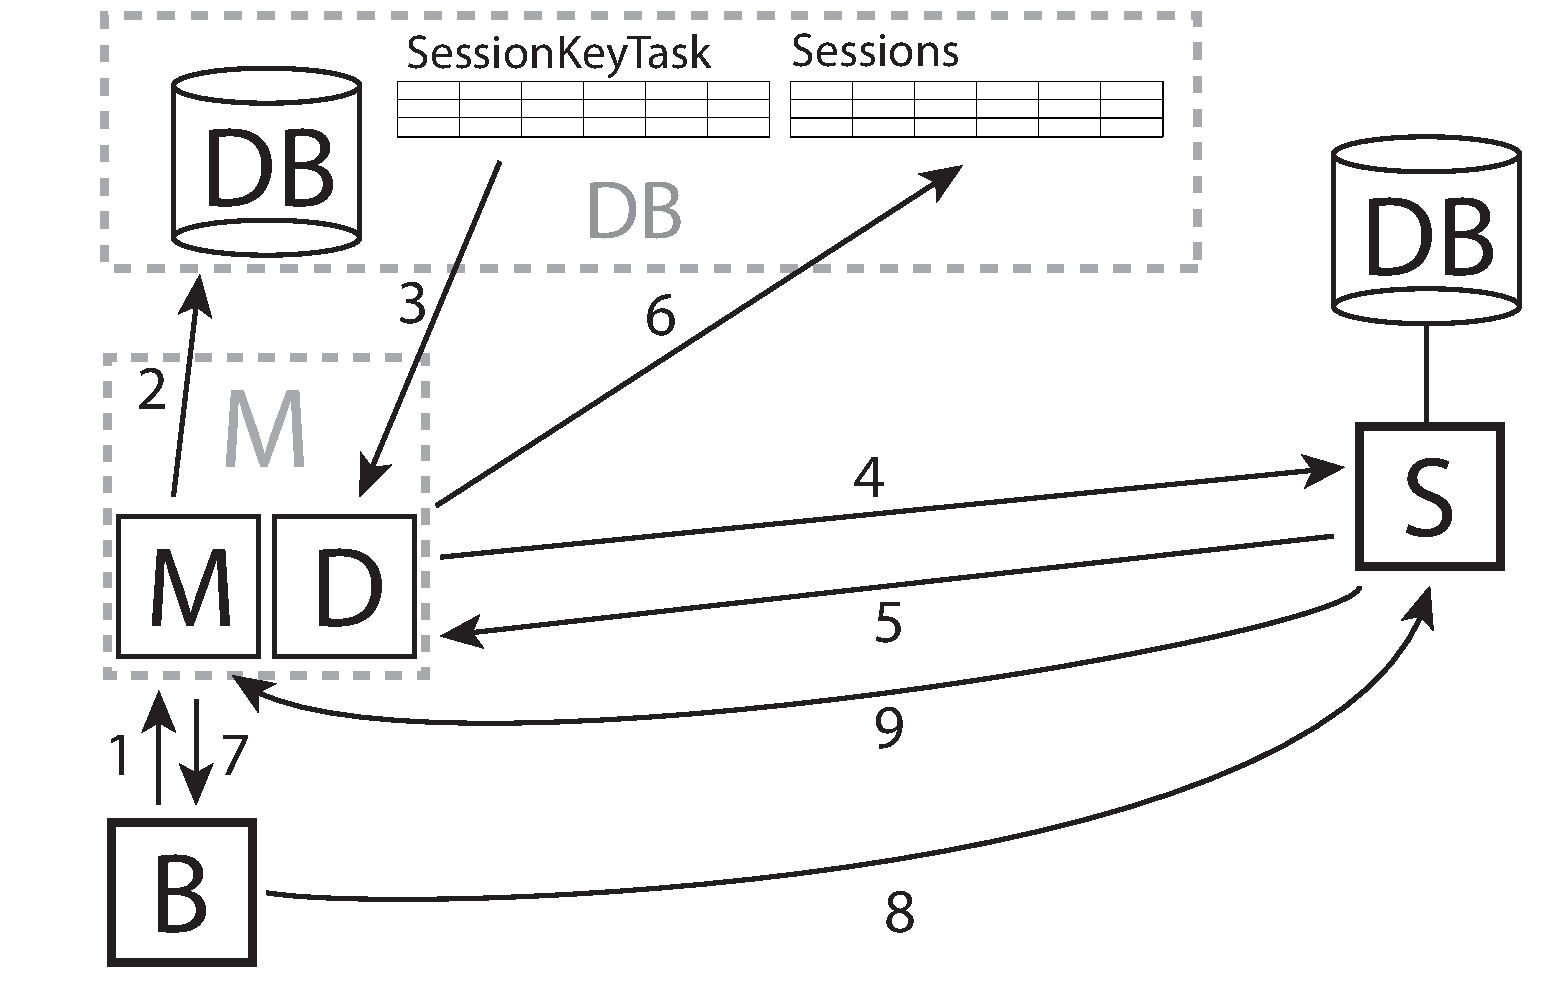
\includegraphics[width=\textwidth]{gfx/sessionkey_communication.pdf}
    \caption{Session key communication between B, M, and S}
    \label{fig:sessionkey_communication}
\end{figure}

This can be seen in figure~\ref{fig:sessionkey_communication}. Session keys have been designed for security. If there did not exist session keys in the system it is possible to highjack a drone.

\begin{enumerate}
	\item Request from B to M to get a session key to view or fly a drone.
	\item M inserts this request in its database table called SessionKeyTask
	\item D scans the database table SessionKeyTask, when it sees a new entry it select it and then deletes it from the table.
	\item D then contacts the S which have the relationship with the drone whom have been requested access to.
	\item S makes a random generated string and uses this as the session key. S updates its own database with this session key and then sends it back to D on M.
	\item D inserts the newly received session key into the session table of M.
	\item M then contacts B with the session key.
	\item B uses this session key to access S and through it the drone.
	\item A Timeout happens if B and S does not communicate for 10 seconds.
\end{enumerate}


\begin{figure}[htb]
    \centering 
    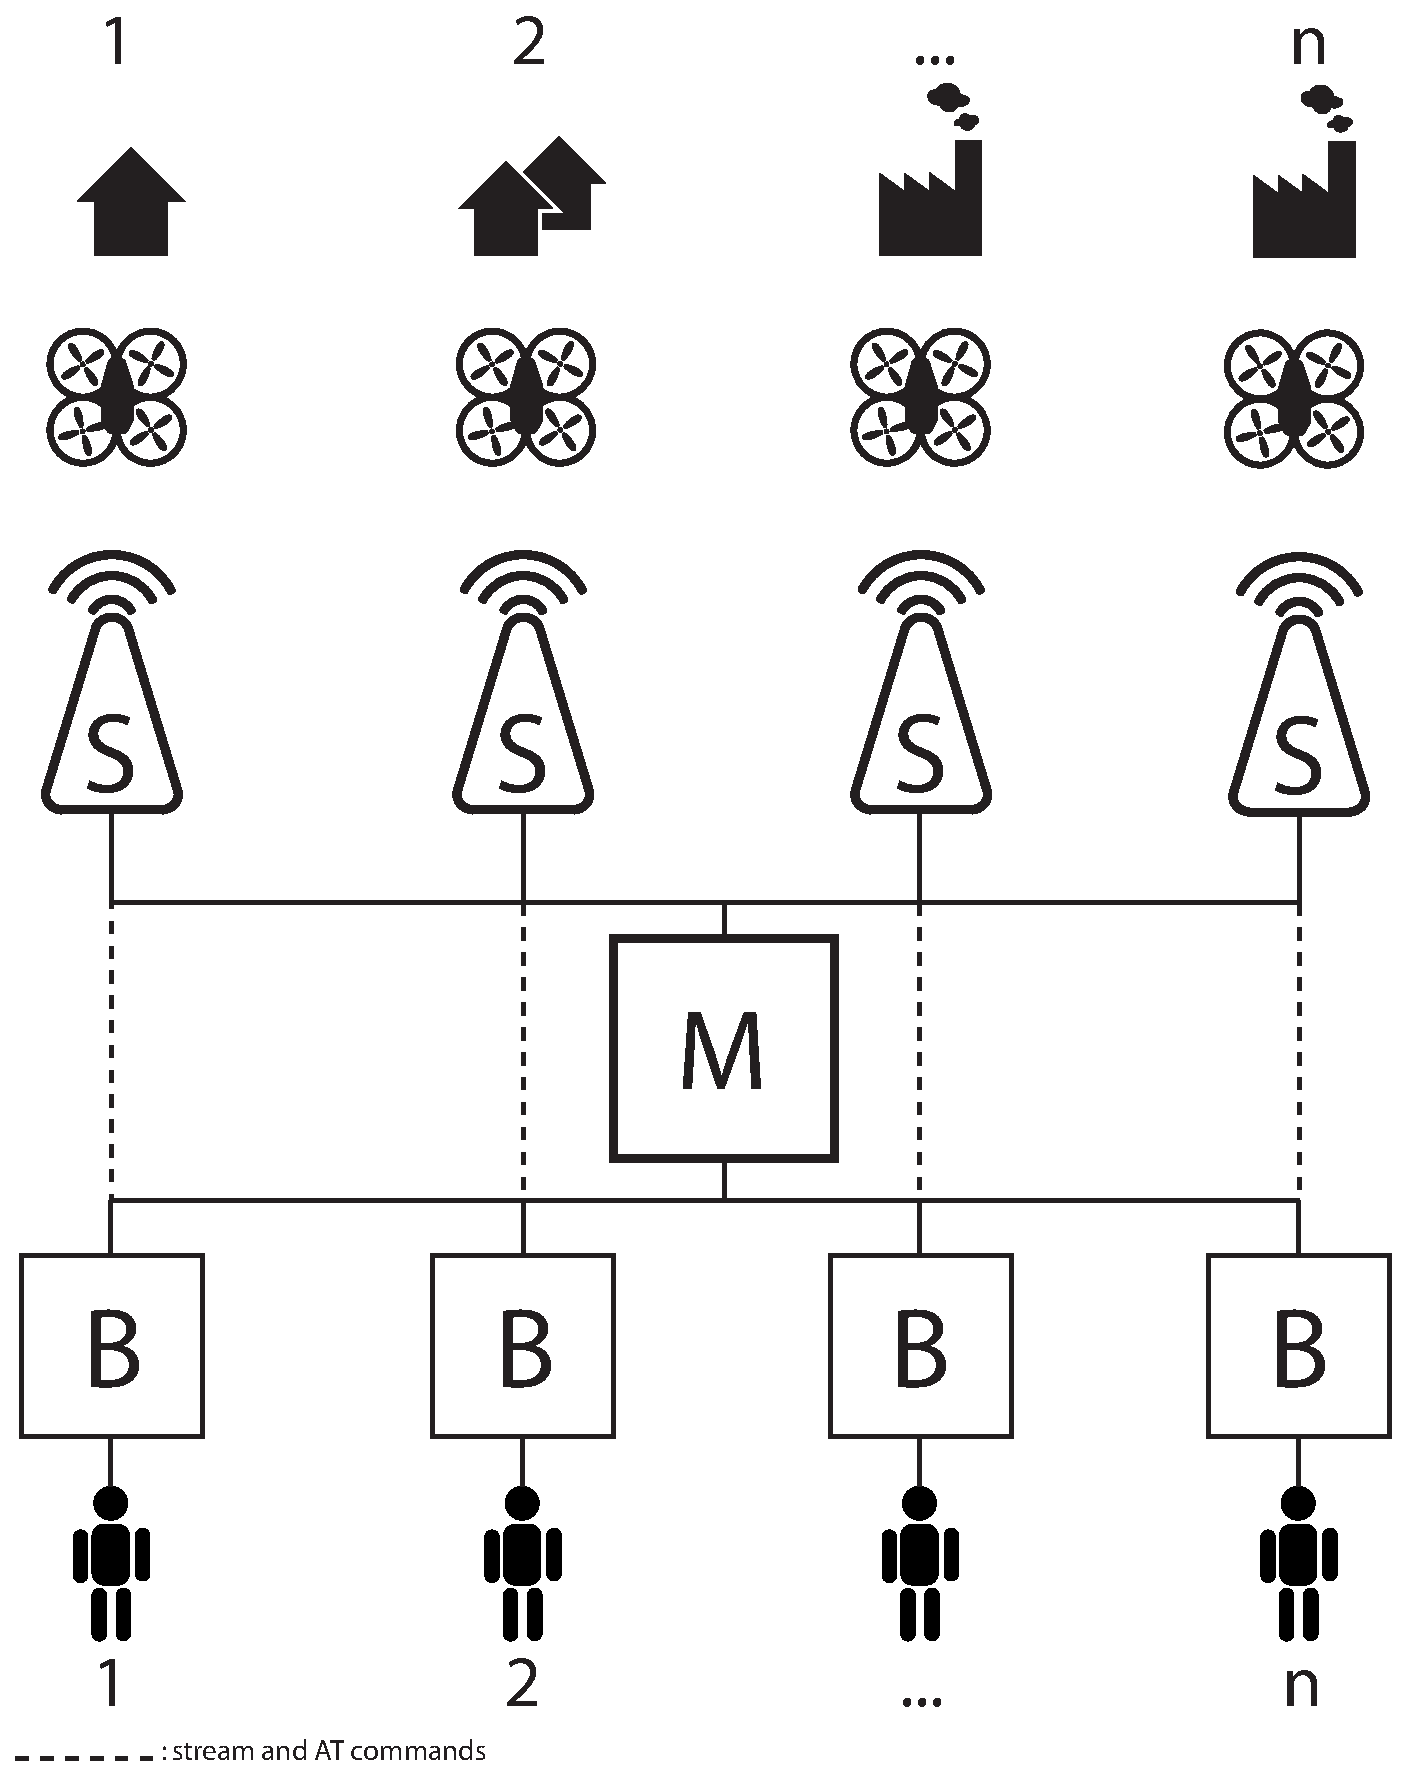
\includegraphics[width=\textwidth]{gfx/system_architecture.pdf}
    \caption{System architecture of \projectname{}}
    \label{fig:system_architecture}
\end{figure}


(Why is this different from other web applications)

\subsection{Master M}

(Only one M?)

\subsection{Slave S}

(More S's?)

\subsection{Daemons}

